\documentclass[conference, 11pt]{IEEEtran}
\IEEEoverridecommandlockouts
% The preceding line is only needed to identify funding in the first footnote. If that is unneeded, please comment it out.
\usepackage{cite}
\usepackage{amsmath,amssymb,amsfonts}
\usepackage{algorithmic}
\usepackage{graphicx}
\usepackage{textcomp}
\usepackage{xcolor}
\def\BibTeX{{\rm B\kern-.05em{\sc i\kern-.025em b}\kern-.08em
    T\kern-.1667em\lower.7ex\hbox{E}\kern-.125emX}}

%Removing indentation.
\newlength\tindent
\setlength{\tindent}{\parindent}
\setlength{\parindent}{0pt}
\renewcommand{\indent}{\hspace*{\tindent}}
\usepackage{float}

\begin{document}

\title{Rain Detection Measurement System Using Infrared Transceiver\\
{\footnotesize \textsuperscript{}ELEN4006}
}

\author{\IEEEauthorblockN{1\textsuperscript{st} Darren Blanckensee}
\IEEEauthorblockA{\textit{School of Electrical and Information Engineering} \\
\textit{University of the Witwatersrand}\\
Johannesburg, South Africa \\
1147279@students.wits.ac.za}
\and
\IEEEauthorblockN{2\textsuperscript{nd} Uyanda Mphunga}
\IEEEauthorblockA{\textit{School of Electrical and Information Engineering} \\
\textit{University of the Witwatersrand}\\
Johannesburg, South Africa \\
1168101@students.wits.ac.za}
}

\maketitle

\begin{abstract}

\end{abstract}

\begin{IEEEkeywords}

\end{IEEEkeywords}

\section{Introduction}
\IEEEPARstart{T}{he} purpose of this project is design and simulate a rain detection measurement system for an electric vehicle. The system is to be mounted under the rear view mirror and uses an infrared transmitter and receiver pair to determine the amount of water on the section of the windshield that is observable by the measurement system. It is a fair assumption that if the amount of water on any section of the windshield is representative of the amount of water on the whole windshield.  This measurement systems purpose is not only to display to the driver how much water is on the windshield and by extension how hard it is raining but also to be able to generate an input to the PWM system that controls the speed of the windshield wipers. The measurement system's design is based on the fundamental principles of measurement systems and the model given in Bentley \cite{BENT}. There are four main sections to this measurement system, namely the sensing stage, the signal conditioning stage, the signal processing stage and the data presentation stage. \\


The sensing stage involves the infrared transmitter and receiver pair. The signal conditioning stage includes the filter which acts as a noise removal filter as well as an anti-aliasing filter. The signal processing stage takes place within the ADC where voltages are related to different levels of rain and the corresponding outputs to the user and the windshield PWM are produced. The smartness of the system is in the ability to calibrate at will which can be used as a means of customising the speed at which the windshield wipers operate as different drivers may have different preferences as to how different levels of rain relate to to certain speeds. The value of this measurement system is that it reduces the number of distractions that occur during the driving process. Driving in the rain is dangerous and having to monitor and adjust the windshield wipers manually is an unnecessary distraction that will with the help of this measurement system be eliminated. Furthermore this report details the static and dynamic characteristics of the designed measurement system. Lastly the Strengths Weaknesses Advantages and Threats~(SWAT) of the measurement system are evaluated and the conclusion then summarises the key points from each section and analyses the successes and failures of this design. 

\section{Background}
	
	
	
\subsection{Measurement Systems}


	
\subsection{Literature Survey}
The use of infrared transceivers (transmitter receievr pairs) in rain detection is not new and has been around since 1958 \cite{SENS}. There are a number of ways to detect rain on the windshield of a car. This report focuses on the use of an infrared transceiver. In \cite{NOTE} the use of a Greenpak SLG46620V integrated circuit in conjunction with the infrared transmitter and receiver allows for great control of a number of characteristics of the measurement system. This was seen as being too complex and did not leave much to design however the transmitter and receiver circuits used in this report are loosely based on those in \cite{NOTE}. 
Furthermore in \cite{NOTE} it is suggested that a single order low pass filter be used at the output however it became clear during the design process that this was not sufficient and so a second order filter was chosen. In
\cite{PULSE} a circuit for pulse generation using a microcontroller (PIC16F876-20) is given. This will be used in the transmitter circuit. 


---------------------- NEEEEEEDS MORE --------------------
	
\subsection{Optics and the Use of Total Internal Reflection}
When light passes through a medium and meets a boundary, if the medium on the other side of the boundary has a lower refractive index than the medium the light is already in and the light strikes this boundary with an angle greater than the critical angle the light is totally internally reflected. When the refractive index of the medium on the other side of the boundary is greater then some of the light is refracted out of the medium and less light is therefore internally reflected. \\

This measurement system takes advantage of this physical phenomenon by shotting infrared light into the windshield at an angle higher than the critical angle calculated to be $41.08 ^{\circ}$ given that the refractive index of air is $1.0003$ and using the average refractive index of windshield glass determined in \cite{RI} to be approximately $1.522$. When there is water on the glass the refractive index on the outside boundary changes from $1.0003$ to $1.333$ which changes the critical angle from $41.08 ^{\circ}$ to $61.14 ^{\circ}$. It is therefore decided that the infrared light be shot at the windshield at an angle of $45 ^{\circ}$ such that when there is no water the light will be totally internally refracted but when water is present the some of the light will be refracted and the received amount of light will be less than what was sent indicating the presence of water. This concept is clearly illustrated in the system block diagram in the Design section below. 

	
\subsection{Real World Simulation (Noise business and real components)}

---------------------- NEEEEEEDS MORE -------------
\cite{NOISE}
	
\section{Design}
This section deals with the design of each of each of the stages shown in the system block diagram in figure 1 that form part of this measurement system. 

 \begin{figure}[H]
 \centering 
 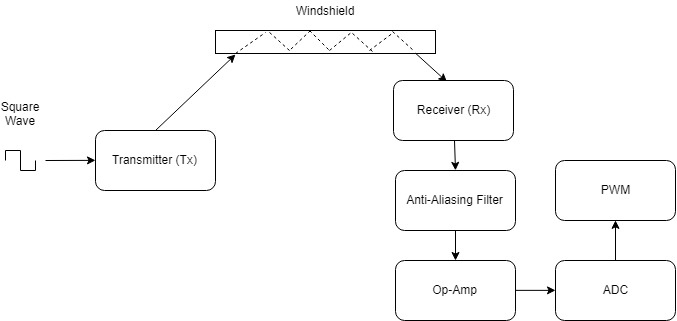
\includegraphics[width=\columnwidth]{SystemBlockDiagram}
 \centering 
  \caption {System block diagram. }
 \end{figure}
 
 Each of these blocks fall into one of the predefined stages in the Bentley model and are explained in depth in the subsections to follow.
 
 \subsection{Transmitter}
 The Infrared transmitter chosen for this system was the IR928-6C-F. It was chosen for its Peak wavelength $λp=940nm$ (chosen because it matches the receivers emitter wavelength) and its low forward voltage of $1.2V$. The transmitter circuit is setup as a typical LED driver circuit with the LED being replaced by the infrared transmitter and the voltage source is replaced by the pulse generator described in the literature review section above. This pulse generator has a period of $1ms$ and a pulse width of $10\mu s$ The Darlington NPN transistor TIP121 was also used. The circuit can be seen in the full system circuit diagram in the appendix. The need for a pulse generator is due to the operating temperature range of the transistor used. If the transistor is on 100\% of the time the power dissipated is 4W which leads to an operating temperature of $275 ^{\circ}C$ which is $125 ^{\circ}C$ above the temperature range specified in the datasheet \cite{TP121}. Therefore it was decided that the pulse generator be used to ensure a duty cycle of 1\% which leads to an operating temperature of $27 ^{\circ}C$ which falls well within the specified range. The output of the transmitter circuit is the voltage difference across the infrared transmitter that produces the infrared light that is shot into the windshield. Graphs of this output can be seen in the simulations section. 

\subsection{Receiver}
The receiver used in this system was the CNY70 reflective optical sensor. It was chosen for its emitter peak wavelength of $940 nm$ which is exactly the same as the peak wavelength of the transmitter and so the light sent by the transmitter will definitely be received by the receiver. The receiver circuit can be seen in the appendix. When light is received by the receiver current is allowed to flow through the circuit which through a resistor produces a voltage. This voltage at the output is expected to be very close to that of the output of the transmitter if there is no rain on the windshield. In the real world however, the matter is not that simple as there is a significant amount of infrared noise in the environment and this needs to be catered for by the system. Due to this when modeling the circuit a noise source was added as the supply to another transmitter circuit that would also be picked up at the receiver just as it would be in the real world. The output of the receiver is a shifted pulse depending on the amount of light received this DC component of the signal can vary between 1 and 6.5 Volts (maximum should be 5V but simulations show noise can shift the signal by as much as 1.5V). These values (1 and 5  Volts) are to be stored by the Microcontroller used in the ADC stage as the values corresponding to heavy rain and no rain respectively. Graphs of the receivers output with rain and without can be seen in the simulations section. 

\subsection{Anti-Aliasing}
In any system that is to be converted from analog to digital it is important to have an Anti-Aliasing filter so as to avoid signal distortion introduced by sampling the signal \cite{FILT}. In this system the output of the signal as shown by the simulations contains a large amount of noise which is not ideal and needs to be dealt with and the authors saw the anti-aliasing filter as an opportunity to deal with the noise while simultaneously catering for the aliasing issues that would otherwise be introduced in the sampling stage. The filter used is a second order low pass filter in Sallen-Key topology with a band pass frequency of $2000Hz$ which is twice the frequency of the pulse at the receiver. The noise is very high frequency and will therefore be eliminated. The circuit for this filter is shown as part of the full circuit diagram in the appendix. The output of the filter is a relatively straight line that resides within a certain voltage range that relates to the amount of water on the windshield. The higher the voltage the less infrared light was lost which means not a lot of water was present on the windshield. The bode plot of the filter is shown in figure 2 below. 

 \begin{figure}[H]
 \centering 
 \includegraphics[width=\columnwidth]{Bode}
 \centering 
  \caption {System block diagram. }
 \end{figure}


\section{Simulation Results}



\section{SWAT Analysis}



\section{Conclusion}



\begin{thebibliography}{22}

	%Each item starts with a \bibitem{reference} command and the details thereafter.

\bibitem{BENT} 
John P. Bentley. \\
\textit{Principles Of Measurement Systems Fourth Edition}. \\
Pearson Education Limited 1983, 2005



\bibitem{SENS} 
Alexandru Vasile, Irina Vasile, Adrian Nistor, Luige Vladareanu, Mihaela Pantazica, Florin Caldararu, Andreea Bonea, Andrei Drumea, Ioan Plotog.\\
\textit{Rain sensor for automatic systems on vehicles}. \\
Proc. SPIE 7821, Advanced Topics in Optoelectronics, Microelectronics, and Nanotechnologies V, 78211W (4 December 2010)

\bibitem{NOTE} 
Dialog Semiconductor. \\
\textit{Application Note IR Windshield Rain Sensor AN-1219}. \\
CFR0014 2 of 23 © Dialog Semiconductor, 2018.


\bibitem{RI} 
Crystal Munger,1 M.S.F.S.; Kris M. Gates,2 B.S., M.A.T.; and Christopher Hamburg,2 B.S. \\
\textit{Determining the Refractive Index Variation within Panes of Vehicle Windshield Glass}. \\
J Forensic Sci, September 2014, Vol. 59, No. 5.



\bibitem{NOISE} 
Łukasz Ciura, Andrzej Kolek, Waldemar Gawron, Andrzej Kowalewski, Dariusz Stanaszek.\\
\textit{MEASUREMENTS OF LOW FREQUENCY NOISE OF INFRARED PHOTO- DETECTORS WITH TRANSIMPEDANCE DETECTION SYSTEM}. \\
METROLOGY AND MEASUREMENT SYSTEMS\\
2014 Polish Academy of Sciences.



\bibitem{PULSE} 
Miloslav HRUŠKOVIC, Ján HRIBIK \\
\textit{Pulse Generator Controlled by Microcontroller}. \\
1 Dept. of Radio Electronics, Slovak University of Technology, Ilkovičova 3, 812 19 Bratislava, Slovak Republic


\bibitem{TP121} 
DARLINGTON TIP120, TIP121, TIP122 (NPN); TIP125, TIP126, TIP127 (PNP)\\
\textit{Plastic Medium-Power Complementary Silicon Transistors}. \\
On Semiconductor


\bibitem{FILT} 
Stefano Bregni, Franco Setti .\\
\textit{Impact of the Anti-Aliasing Pre-Filtering on the Measurement of Maximum Time Interval Error}. \\
0-7803-4198-8/97/\$10.00 0 1997 IEEE





\end{thebibliography}
\end{document}
